\documentclass[11pt]{article}
\usepackage{amsmath, amssymb, array}
\pagestyle{plain}

\textwidth=6.5in
\hoffset-1in
\textheight=9in
\voffset-1in

\usepackage{enumitem}
\usepackage{pgfplots}
\usepackage{graphicx}
\usepackage{lipsum}
\usepackage{stfloats}
\usepackage{multicol}
\setlength{\columnsep}{1cm}




\begin{document}


\noindent MATH 1113   \hfill 4.4 - Trigonometric Functions of Any Angle\\



\noindent \textbf{Topics:}  increasing and decreasing, reference angles\\

\noindent \textbf{Student Learning Outcomes:}
\begin{enumerate}
\item Students will be able to evaluate trigonometric functions of any angle.
\item Students will be able to determine reference angles.
\item Students will be able to evaluate trigonometric functions using reference angles.
\end{enumerate}

\hrule 
\vspace{5mm}
\section{Trigonometric Functions of Any Angle}
\noindent  Recall:  We have used trigonometric functions with acute angles.  What if the angle is not acute?\vfill

\noindent A circle with center $(0,0)$ and radius $r$ has the equation $x^2+y^2=r^2$.  Choose a point $P(x,y)$.  We can create reference triangles inside the circle in order to define our trig functions.\\[2.5in]


\noindent If the point $(x,y)$ lies on the \textbf{terminal side} of $\theta$, the six trig functions of $\theta$ can be defined as follows:

$$\sin(\theta)=\frac{y}{r} \quad \quad \quad \quad \quad \quad \cos(\theta)=\frac{x}{r} \quad \quad \quad \quad \quad \quad \tan(\theta)=\frac{y}{x} $$

$$\csc(\theta)=\frac{r}{y} \quad \quad \quad \quad \quad \quad \sec(\theta)=\frac{r}{x} \quad \quad \quad \quad \quad \quad \cot(\theta)=\frac{x}{y} $$
\vfill
\noindent What changes when we are on the unit circle?



\newpage



\begin{enumerate}
\item Let $P(-6,8)$ be a point on the terminal side of $\theta$.  Find each of the six trig functions of $\theta$.\\[2in]

\begin{center}
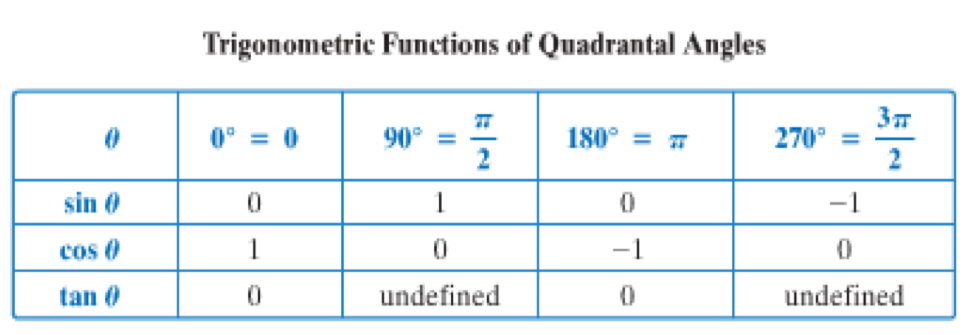
\includegraphics[scale=.7]{quadrantal}
\end{center}

\section{The Signs of the Trigonometric Functions}
\begin{center}
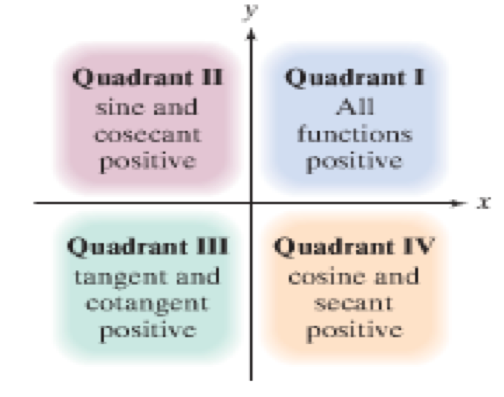
\includegraphics[scale=.8]{signs}
\end{center}

\item Let $\theta$ be an angle in standard position.  Name the quadrant in which $\theta$ lies.
$$\sin(\theta)<0, \quad \quad \tan(\theta)<0$$


\newpage

\item Find the exact value of each of the remaining trigonometric functions of $\theta$.
$$\sin(\theta)=\frac{4}{5}, \quad  \theta \text{ in Quadrant 2}$$\vfill


\section{Reference Angles}

Let's draw our two reference triangles as well as an $xy-$plane.\\[1.5in]
\hspace{-.3in}\begin{tabular}{| l |} \hline
Let $\theta$ be a nonquadrantal angle in standard position. The \underline{reference angle} for $\theta$, \\ called $\theta_R$, is the \emph{acute} angle $\theta_R$ that the \emph{terminal side} of $\theta$ makes with the $x$-axis. \\ \hline
\end{tabular}\\
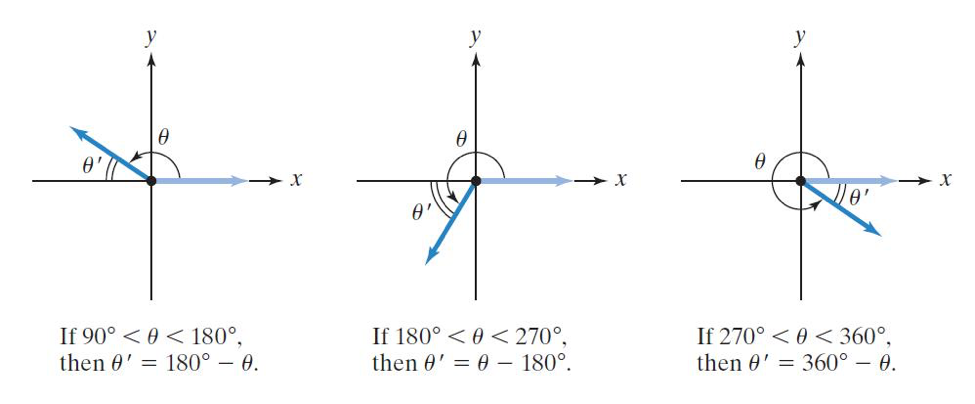
\includegraphics{refimage}\\

\newpage

\item Determine the reference angle $\theta_R$ for each of the following angles.
\begin{enumerate}
\item $\theta = 45^\circ$ \hspace{1in} Quadrant \underline{\phantom{sldkjfslkdjf}} \hspace{1in} $\theta_R$ \underline{\phantom{sldkjfslkdjf}} \\[.8in]
\item $\theta = -73^\circ$ \hspace{1in} Quadrant \underline{\phantom{sldkjfslkdjf}} \hspace{1in} $\theta_R$ \underline{\phantom{sldkjfslkdjf}}  \\[.8in]

\item $\theta = -915^\circ$ \hspace{1in} Quadrant \underline{\phantom{sldkjfslkdjf}} \hspace{1in} $\theta_R$ \underline{\phantom{sldkjfslkdjf}}  \\[.8in]

\end{enumerate}

\item Determine the reference angle $\theta_R$ for each of the following angles. 
\begin{enumerate}

\item $\theta = \dfrac{19\pi}{6}$ \hspace{1in} Quadrant \underline{\phantom{sldkjfslkdjf}} \hspace{1in} $\theta_R$ \underline{\phantom{sldkjfslkdjf}} \vfill
\item $\theta = \dfrac{47\pi}{4}$ \hspace{1in} Quadrant \underline{\phantom{sldkjfslkdjf}} \hspace{1in} $ \theta_R$ \underline{\phantom{sldkjfslkdjf}} \vfill
\item $\theta = \dfrac{-7\pi}{6}$ \hspace{1in} Quadrant \underline{\phantom{sldkjfslkdjf}} \hspace{1in} $\theta_R$ \underline{\phantom{sldkjfslkdjf}} \vfill

\end{enumerate}

\newpage


\hspace{-.3in}\begin{tabular}{| l |} \hline
Let $\theta$ be a nonquadrantal angle in standard position. To find the value of a trig function\\ at $\theta$, find its value for the \emph{reference angle} $\theta_R$ and prefix the appropriate sign (using ASTC). \\ \hline
\end{tabular}

\item Determine the exact values of $\sin(2\pi/3)$ and $\cos(2\pi/3)$. \\[1.5in] %QII


\item Determine the exact values of $\cos(210^\circ)$, $\sec(210^\circ)$, and $\cot(210^\circ)$. \\[1.5in]
\vfill
%
%\item Determine the exact value of each of the following. %same ref
%\begin{enumerate}
%\item $\sin(7\pi/6)$ \vfill
%
%\item $\sin(11\pi/6)$ \vfill
%\item $\sin(5\pi/6)$ \vfill
%\end{enumerate}
%
%
%\newpage
%\item Suppose $\theta$ is an angle in the third quadrant with reference angle $\theta_R$ satisfying $\cos(\theta_R)=5/13$ and $\sin(\theta_R)=12/13$.  Determine the exact values of $\cos(\theta)$ and $\csc(\theta)$.  \vfill


\end{enumerate}

\noindent \textbf{Student Learning Outcomes Check}

\begin{enumerate}
\item Can you evaluate trigonometric functions of any angle?
\item Are you able to determine reference angles?
\item Can you evaluate trigonometric functions using reference angles?
\end{enumerate}

\noindent \textbf{If any of your answers were no, please ask about these topics in class.}













\end{document}